\documentclass[11pt,spanish]{article}
\usepackage[spanish]{babel}
\selectlanguage{spanish}
\usepackage[utf8]{inputenc}
\usepackage{graphicx}
\usepackage{caption}
\usepackage{subcaption}
\usepackage{hyperref}

\begin{document}

\title{Redes Neuronales Profundas: Trabajo Práctico 1}
\date{}
\maketitle

\section*{Respuestas}
El código realizado para la resolución de los ejercicios está disponible en \href{https://github.com/dncampo/deep-learning/tree/lpineda}{github} (branch \textit{lpineda})

\subsection*{Ejercicio 1}
Para leer el dataset completo se genera recursivamente una lista de \textit{strings} con las rutas de las imágenes. Luego, estas son leídas utilizando la función \textit{reshape\_image}, la cual descarta una fila o una columna si el alto o el ancho tienen dimensiones impares, y centra la imagen en un rectángulo negro de las medidas dadas.
Dado que el dataset completo no cabe en memoria, solo se lee un subdirectorio elegido al azar para realizar las pruebas.

\subsection*{Ejercicio 2}
En este ejercicio se toman imágenes directamente del dataset, sin el procesamiento realizado en el ejercicio 1. Dado que se deben extraer parches en posiciones aleatorias de la imagen, la subimagen podría ser seleccionada de uno de los bordes negros, lo cual no agregaría información relevante. Como el tamaño de los parches es muy pequeño, no se incluye ninguna captura. La función está implementada con el nombre \textit{extract\_window}.

Por otro lado, para normalizar la imagen con $\mu=0$ y $\sigma^2=1$, a cada pixel de la imagen se le sustrae la media y se lo divide por la desviación estandar. Esto es, para una imagen $I$: 

\begin{center}
	\begin{math}
	\forall p_{i,j} \in I, \qquad \hat{p}_{i,j} = \frac{(p_{i,j} - \mu_I)}{\sigma^2_I}
	\end{math}
\end{center}

El resultado de este procesamiento se puede observar en la figura \ref{normalized_img}. La imagen transformada es inteligible puesto que al normalizar cada canal, los valores enteros de los pixeles en el rango $[0,255]$ son transformados a valores flotantes, y al tener una distribución de probabilidad con $\mu=0$ es de esperar la existencia de valores negativos. Estos son casteados a enteros por la librería utilizada\footnote{Python Imaging Library (PIL): http://www.pythonware.com/products/pil/}. \par

\begin{figure}[htbp]
	\centering
	\begin{minipage}[b]{0.35\textwidth}
		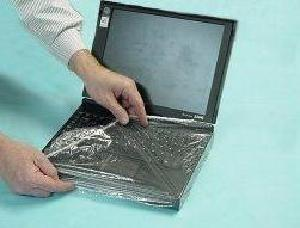
\includegraphics[width=\textwidth]{../image.jpg}
		\caption{Imagen original.}
		\label{original_img}
	\end{minipage}
	\hfill
	\begin{minipage}[b]{0.35\textwidth}
		
\includegraphics[width=\textwidth]{../normalized_image.jpg}
		\caption{$\mu=0 \quad \sigma^2=1$}
		\label{normalized_img}
	\end{minipage}
\end{figure}

Sin embargo, el hecho que la imagen sea inteligible no quiere decir que la información se haya perdido. Esto se puede comprobar al transformar los valores de los pixeles al rango $[0,255]$ mediante la función:
\ \
\begin{center}
	\begin{math}
		f(x) = int\lbrace 255 \frac{x-min(I)}{max(I)-min(I)} \rbrace
	\end{math}
\end{center}
donde nuevamente $I$ es una imagen dada. Esta función está implementada bajo el nombre \textit{quantize}, y el resultado de su aplicación a los pixeles de la imagen \ref{normalized_img} (en su versión de valores flotantes) puede observarse en la figura \ref{quantized_img}.

\begin{figure}[htbp]
	\centering
	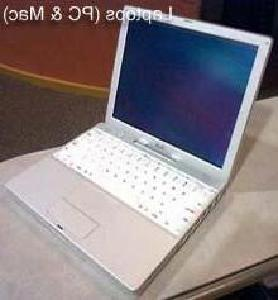
\includegraphics[width=0.35\textwidth]{../quantized_image.jpg}
	\caption{Imagen cuantizada}
	\label{quantized_img}
\end{figure}

Si bien a primera vista las imágenes originales y transformadas pueden parecer iguales, en base al histograma podemos observar que la transformación aplicada hace que la distribución de los pixeles varíe en cada canal, siendo la segunda más uniforme.

\begin{figure}[htbp]
	\centering
	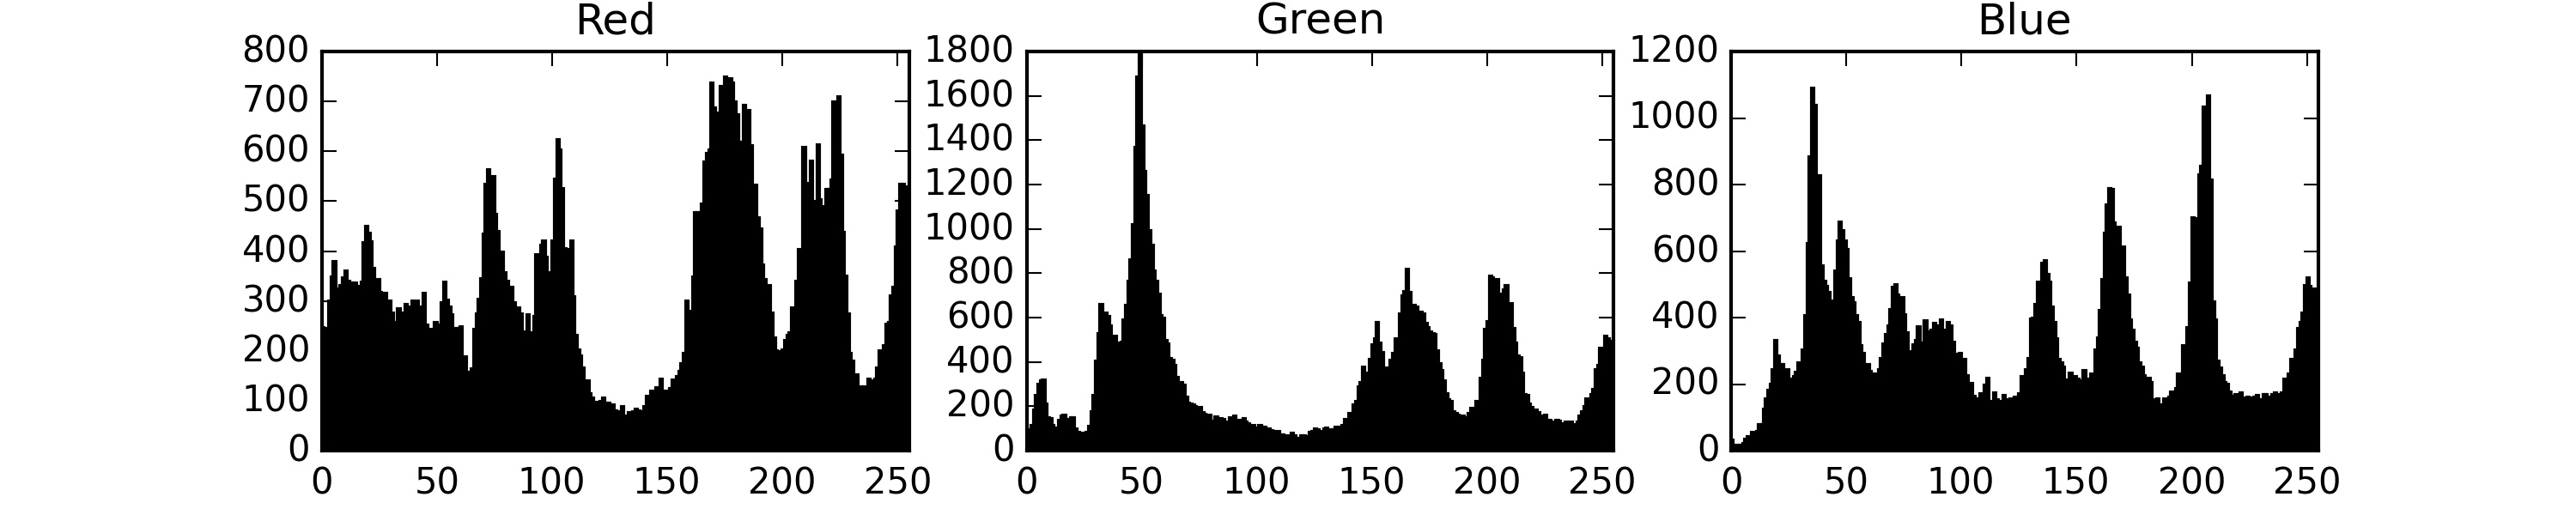
\includegraphics[width=1\textwidth]{../image_histogram.jpg}
	\caption{Histograma de la imagen original}
	\label{hist_original_img}
\end{figure}

\begin{figure}[htbp]
	\centering
	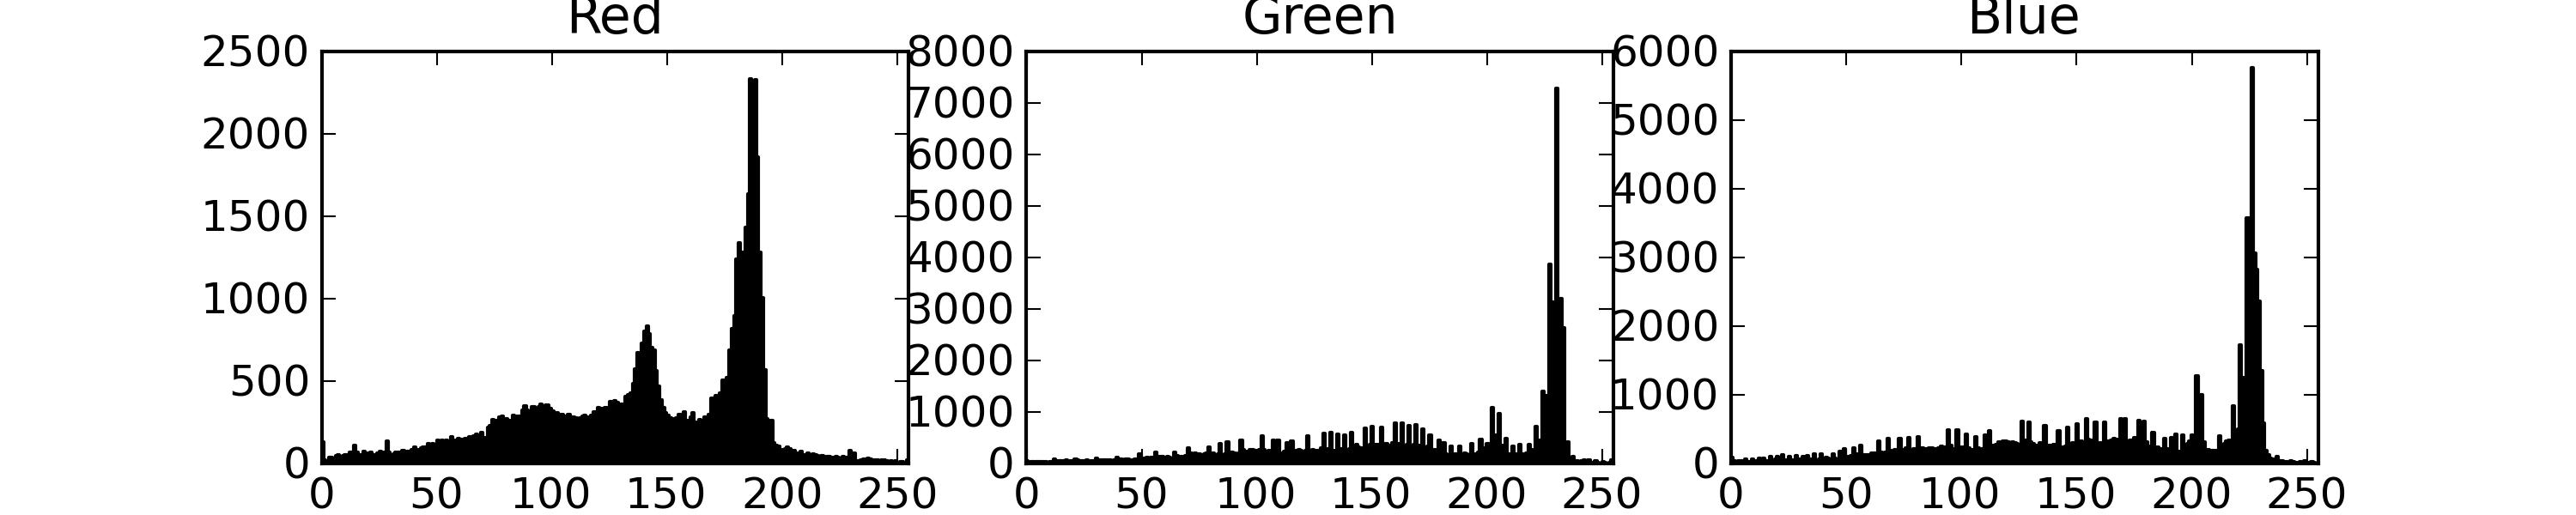
\includegraphics[width=1\textwidth]{../quantized_image_histogram.jpg}
	\caption{Histograma de la imagen cuantizada}
	\label{hist_quantized_img}
\end{figure}

\subsection*{Ejercicio 3}
Las imagenes naturales (las imagenes que los humanos estamos acostumbrados a ver, como paisajes, animales, etc) contienen información redundante dada la alta correlación entre pixeles adjacentes. Si utilizamos un dataset de imágenes para entrenar algún modelo, lo ideal sería que las entradas contengan la menor cantidad de información repetida posible; el objetivo de aplicar \textit{whitening} sobre cada imagen de un dataset es hacer que los datos con los que entrenamos la red neuronal no tengan información redundante. \par
Dados $m$ vectores de características $\mathbf{x}$ (nuestro dataset) con media cero $\mu_{\mathbf{x}_i}=0$, la matriz de covarianza está dada por:
\begin{center}
	\begin{math}
		\mathbf{\Sigma} = \frac{1}{m} \sum_{i=1}^{m} \mathbf{x} \mathbf{x}^T
	\end{math}
\end{center}

Si queremos que los datos no estén correlacionados, debemos transformar el dataset de forma que su matriz de covarianza $\mathbf{\Sigma}$ sea una matriz diagonal. Esta transformación se puede expresar lograrse pre-multiplicando cada vector de características por la matriz $\mathbf{\Phi}^T$, donde las columnas de $\mathbf{\Phi}$ son los eigenvectores de la matriz de covarianza $\mathbf{\Sigma}$. Podemos expresar la matriz de covarianza diagonalizada como:

\begin{center}
	\begin{math}
		\mathbf{\Phi}^T \mathbf{\Sigma} \mathbf{\Phi} = \mathbf{\Lambda}
	\end{math}
\end{center}
donde $\mathbf{\Lambda}$ es una matriz de ceros con los eigenvalores de la matriz de covarianza en su diagonal. Luego, la matriz de covarianza de $\mathbf{y} = \mathbf{\Phi}^T \mathbf{x}$ es la matriz diagonal $\mathbf{\Lambda}$. \par
Aplicar \textit{whitening} a un dato consiste en hacer que su matriz de covarianza tenga la forma $\mathbf{\Lambda} = \alpha \mathbf{I}$. Usando el hecho que:

\begin{center}
	\begin{math}
		\mathbf{\Lambda}\mathbf{\Lambda}^{-1} = 1 \rightarrow \mathbf{\Lambda}^{-1} = \mathbf{\Lambda}^{-1/2} \mathbf{I} \mathbf{\Lambda}^{-1/2} \rightarrow  \mathbf{I} = \mathbf{\Lambda}^{-1/2} \mathbf{\Lambda} \mathbf{\Lambda}^{-1/2}
	\end{math}
\end{center}

y reemplazando $\mathbf{\Lambda}$ tenemos que:

\begin{center}
	\begin{math}
	\mathbf{\Lambda}^{-1/2} \mathbf{\Phi}^T \mathbf{\Sigma} \mathbf{\Phi} \mathbf{\Lambda}^{-1/2} = \mathbf{I}
	\end{math}
\end{center}

Finalmente, la transformación $\mathbf{z}$ para \textit{blanquear} los datos esta dada por:
\begin{center}
	\begin{math}
	\mathbf{z} = \mathbf{\Lambda}^{-1/2} \mathbf{\Phi}^T \mathbf{\Sigma} \mathbf{x}
	\end{math}
\end{center}

Esto se puede comprobar al calcular la matriz de covarianza de $\mathbf{z}$
\begin{center}
	\begin{math}
		\mathbf{\Sigma} = \frac{1}{m} \sum_{i=1}^{m} \mathbf{z} \mathbf{z}^T = \
		\frac{1}{m} \sum_{i=1}^{m} \mathbf{\Lambda}^{-1/2} \mathbf{\Phi}^T \mathbf{x} \mathbf{x}^T  \mathbf{\Phi} \mathbf{\Lambda}^{-1/2} = \mathbf{I}
	\end{math}
\end{center}

\subsection*{Ejercicio 4}
Aplicar un procedimiento similar al del ejercicio 2 en las imágenes del dataset de palabras manuscritas produce resultados similares. Aunque el cambio es muy sutil, podemos observar que la imagen normalizada se aclara.

\begin{figure}[htbp]
	\centering
	\begin{minipage}[b]{0.4\textwidth}
		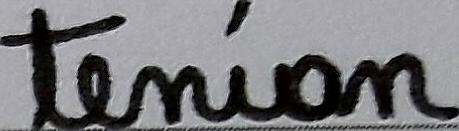
\includegraphics[width=\textwidth]{../words_image.jpg}
		\caption{Imagen original.}
		\label{original_word}
	\end{minipage}
	\hfill
	\begin{minipage}[b]{0.4\textwidth}
		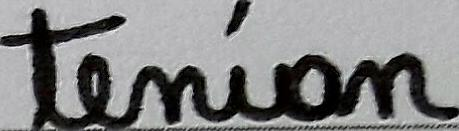
\includegraphics[width=\textwidth]{../words_quantized_image.jpg}
		\caption{$\mu=0 \quad \sigma^2=1$}
		\label{quantized_word}
	\end{minipage}
\end{figure}

Al analizar los histogramas, vemos que los picos con la mayor concentración de pixeles se desplazan a la derecha, lo que resulta en un aumento general de brillo de la imagen.

\begin{figure}[htbp]
	\centering
	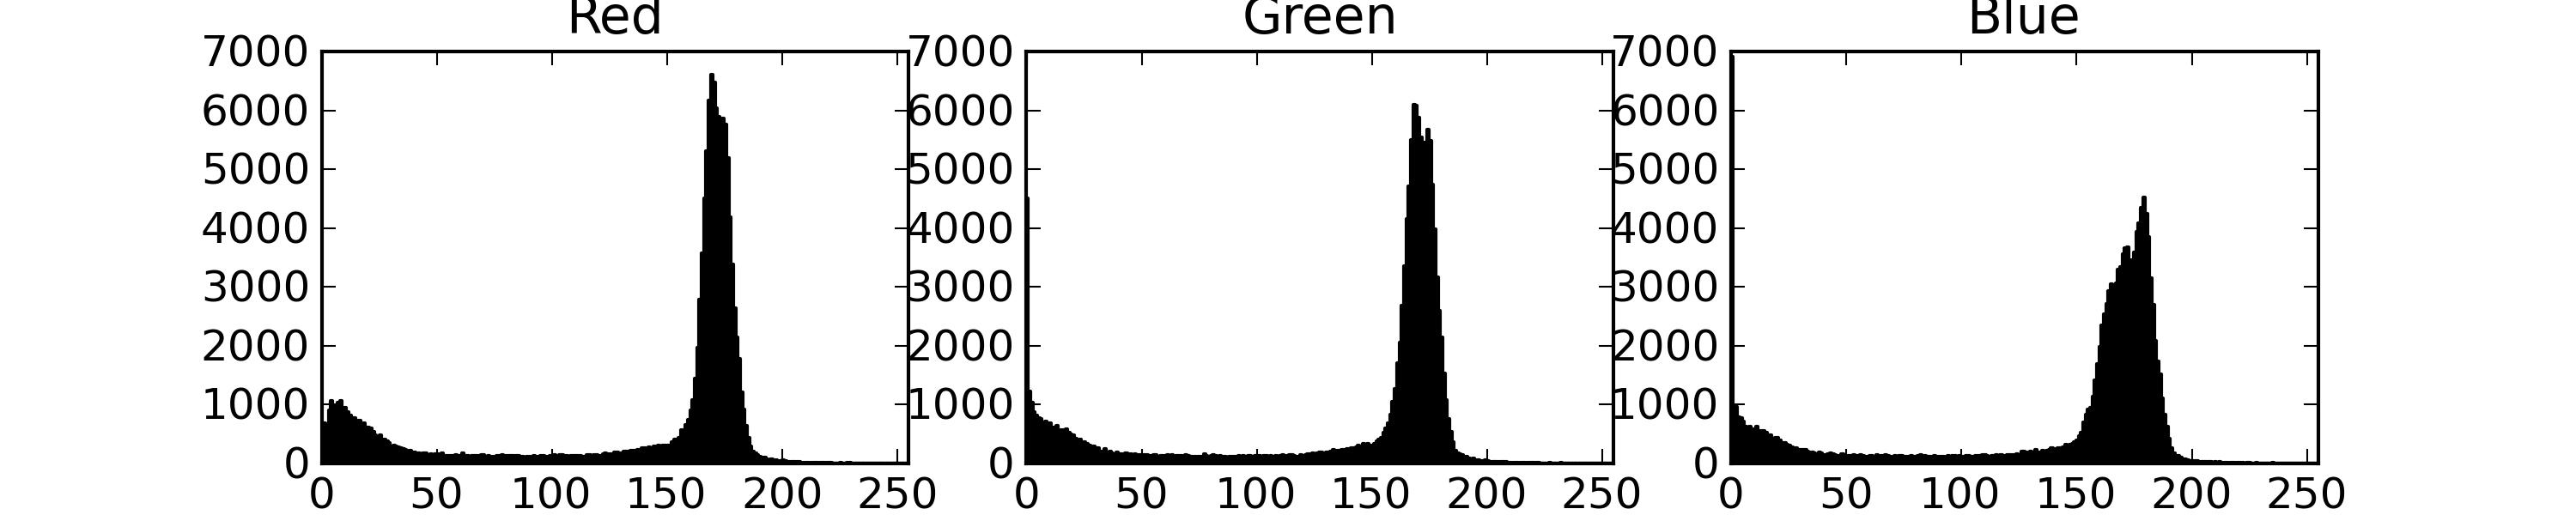
\includegraphics[width=1\textwidth]{../words_image_histogram.jpg}
	\caption{Histograma del texto manuscrito original}
	\label{hist_original_word}
\end{figure}

\begin{figure}[htbp]
	\centering
	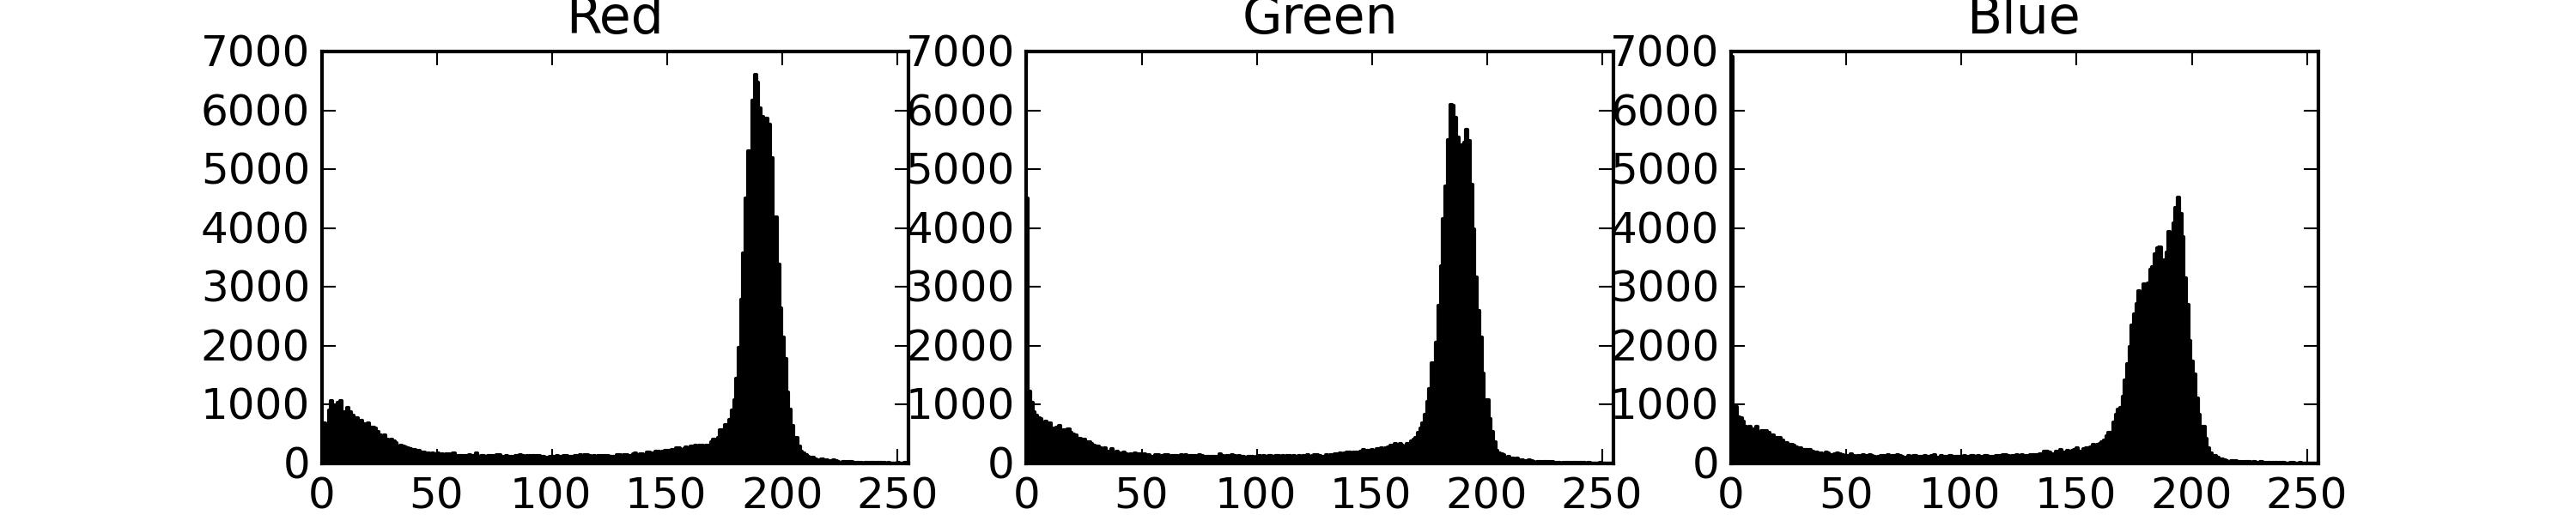
\includegraphics[width=1\textwidth]{../words_quantized_image_histogram.jpg}
	\caption{Histograma del texto manuscrito normalizado y cuantizado}
	\label{hist_quantized_word}
\end{figure}


\end{document}